%!TEX root = ./roll_your_own.tex
\chapter{Variations on the Sequent Calculus}
\label{chap:sequentvariations}

The calculus of \chapref{sequentcalculus} is only one of very many possible variants. In this chapter I discuss the way in which you can encode an LF-style treatment of variables in the quantifier introduction and elimination rules, how Jape deals with non-additive rules, and two versions of the intuitionistic sequent calculus --- multiple and single conclusion.

\word{var,inscope}
\begin{table}
\centering
\caption{LF variables in the multiple-conclusion sequent calculus}
\label{tab:LFvars}
\vstrut{30pt}
$\infer[\reason{(fresh $m$) ⊦∀}]
       {\Gamma |- @*x.A(x),\Delta }
       {\Gamma,\<var> m |- A(m),\Delta } $
\qquad\vstrut{30pt}
$\infer[\reason{⊦∃}]
       {\Gamma  |-|*x.A(x) ,\Delta }
       {\Gamma  |- A(B),\Delta \quad \Gamma |- B\;\<inscope>} $
\qquad\vstrut{30pt}
$\infer[\reason{∀⊦}]
       {\Gamma,@*x.A(x) |- \Delta }
       {\Gamma,A(B)  |- \Delta \quad \Gamma |- B\;\<inscope>}$
\qquad\vstrut{30pt}
$\infer[\reason{(fresh $m$) ∃⊦}]
       {\Gamma ,|*x.A(x)  |- \Delta }
       {\Gamma,\<var> m,A(m)  |- \Delta }$
\end{table}

\section{LF-style variables in quantifier rules}

Jape allows redefinition of any rule, theorem or conjecture\footnote{And it allows it \emph{at any time}!! It ought to check, whenever a rule or theorem is redefined, every proof that relies upon it. It doesn't.}. The file \texttt{examples/MSC\_LF.j} redefines the quantifier rules to allow a more careful treatment of variables\footnote{Explanation for non-expert logicians: the effect is to make it much more careful about the treatment of possibly-empty domains of quantification. It is impossible, for example, to prove $@*x.P(x) |- |*x.P(x)$, because the proof would require that there be some $m$ such that $P(m)$.}. The new rules are shown in \tabref{LFvars}.

The intention is that a variable $c$ is `$\<inscope>$' if there is an assumption $\<var> c$; a formula is $\<inscope>$ if its free variables. Note that there is nothing in Jape which demands that we use these words nor this technique: it's up to the logic decoder to program it.


The file \texttt{sequent\_scoping.j} defines two low priority prefix operators:
\begin{quote}\tt\small
PREFIX  10              var \\
POSTFIX 10              inscope
\end{quote}
and a structural induction to handle formulae,\footnote{This induction is unnecessary: in the sequent calculus we never need anything more complicated than a variable. But I wanted to see if I could do something more general, and I have left it in.} automatically applied whenever there is an open tip:
\begin{quote}\tt\small

RULES "inscope" ARE
\tab       Γ, var x ⊢ x inscope\\
AND     FROM Γ ⊢ A inscope AND Γ ⊢ B inscope INFER Γ ⊢ A→B inscope\\
AND     FROM Γ ⊢ A inscope AND Γ ⊢ B inscope INFER Γ ⊢ A∧B inscope\\
AND     FROM Γ ⊢ A inscope AND Γ ⊢ B inscope INFER Γ ⊢ A∨B inscope\\
AND     FROM Γ ⊢ A inscope INFER Γ ⊢ ¬A inscope\\
AND     FROM Γ, var x ⊢ A inscope INFER Γ ⊢ ∀x.A inscope\\
AND     FROM Γ, var x ⊢ A inscope INFER Γ ⊢ ∃x.A inscope \\
END

\end{quote}

Encoding of the rules is then straightforward in \texttt{MSC\_LF.j}:
\begin{quote}\tt\small
RULE    "⊢∀"(OBJECT m) WHERE FRESH m\\
\tab                    FROM Γ, var m ⊢ A(m),∆                    INFER Γ ⊢ ∀x.A(x),∆\\
RULE    "∀⊢"(B)   FROM Γ, A(B) ⊢ ∆ AND Γ ⊢ B inscope      INFER Γ,∀x.A(x) ⊢ ∆\\
RULE    "⊢∃"(B)   FROM Γ ⊢ A(B),∆ AND Γ ⊢ B inscope       INFER Γ ⊢ ∃x.A(x),∆\\
RULE    "∃⊢"(OBJECT m) WHERE FRESH m\\
\tab                    FROM  Γ, var m, A(m) ⊢ ∆                  INFER Γ, ∃x.A(x) ⊢ ∆\\
\end{quote}
I would like inscope judgements to behave like side conditions, displayed when they are a problem and hidden when they are satisfied. But they aren't provisos, because they relate a particular context and a particular formula.

In order to make these judgements behave like side conditions I use Jape's \textsc{layout} tactical: it allows me to run a tactic and to decide which subtrees of the resulting proof tree should be displayed and what should be written as the justification of the step. (Subtrees which contain open problem sequents are always displayed, so that nothing which might accidentally be important is hidden.) In the case of the ⊦∀ and ∃⊦ rules I would like to display the first antecedent proof (numbered 0) and hide the second (numbered 1); in either case I want to give the name of the rule as the justification of the step. The tactics are
\begin{quote}\tt\small

TACTIC "∀⊢ with side condition hidden" IS LAYOUT "∀⊢" (0) (WITHSELECTIONS "∀⊢")\\
TACTIC "⊢∃ with side condition hidden" IS LAYOUT "⊢∃" (0) (WITHSELECTIONS "⊢∃")
\end{quote}
which I put into the menu, overwriting any previous entries with the same label:
\begin{quote}\tt\small
MENU Rules IS
\tab ENTRY "∀⊢" IS "∀⊢ with side condition hidden"\\
\tab ENTRY "⊢∃" IS "⊢∃ with side condition hidden"\\
END
\end{quote}
and into the list of double-click actions
\begin{quote}\tt\small
HYPHIT  ∀x.A ⊢  IS "∀⊢ with side condition hidden"\\
CONCHIT ⊢ ∃x.B  IS "⊢∃ with side condition hidden"
\end{quote}
You get all this machinery by loading \texttt{MCS.jt}, to get the multiple-conclusion sequent calculus, and then adding \texttt{MCS\_LF.j}, to get the extra rules and syntax.

\begin{figure}
\centering
\fbox{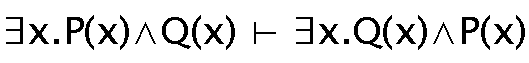
\includegraphics[scale=0.5]{pics/LF0}}\qquad
\fbox{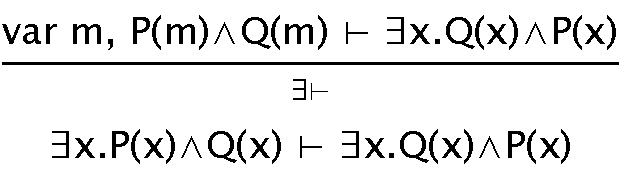
\includegraphics[scale=0.5]{pics/LF1}}\qquad
\fbox{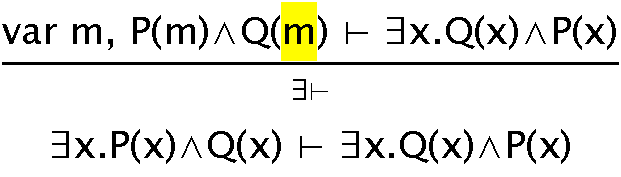
\includegraphics[scale=0.5]{pics/LF1a}}\qquad
\fbox{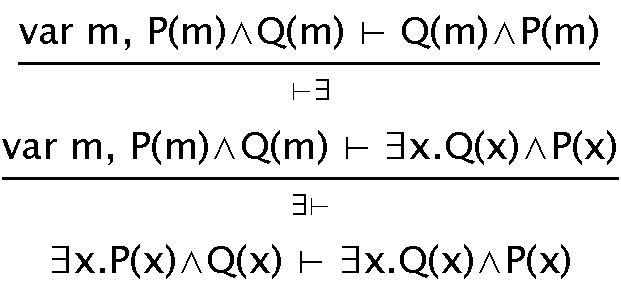
\includegraphics[scale=0.5]{pics/LF2}}\qquad
\caption{Using LF variables in the multiple-conclusion sequent calculus}
\label{fig:LF}
\end{figure}


\begin{figure}
\centering
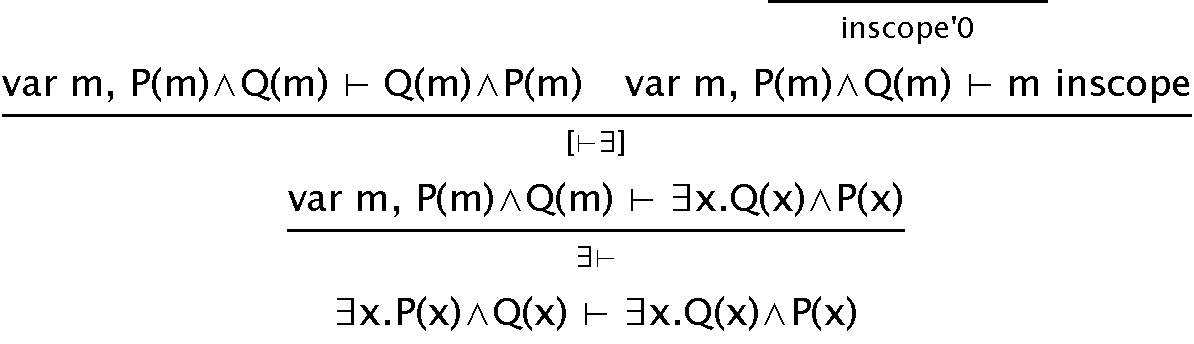
\includegraphics[scale=0.5]{pics/LF2a}
\caption{Hidden antecedents exposed}
\label{fig:LFa}
\end{figure}


Under this encoding, \figref{LF} showsthe progress of a proof in which the variable rules are obeyed. One antecedent of the final step isn't shown. You can see the full tree, shown in \figref{LFa}, by double-clicking on the justification of that step. Clearly it is an advantage to hide the side-proof whenever possible; it makes sense to hide it when it is closed, as in this case.

\begin{figure}
\centering
\fbox{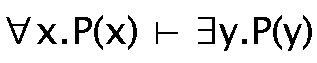
\includegraphics[scale=0.5]{pics/LFbad0}}\qquad
\fbox{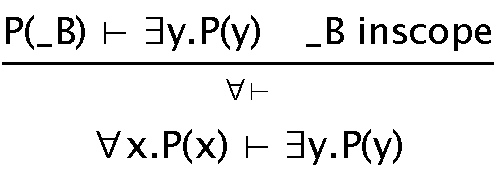
\includegraphics[scale=0.5]{pics/LFbad1}}\qquad
\fbox{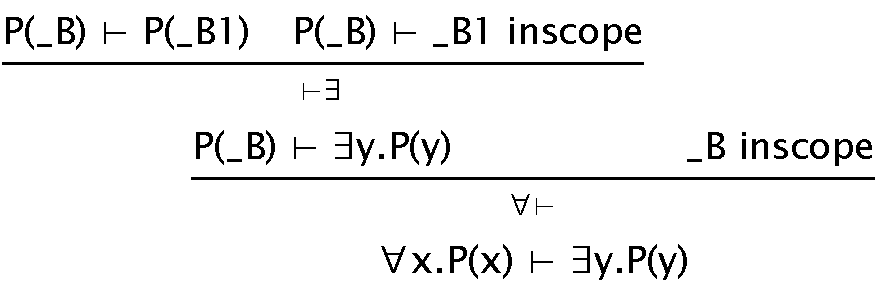
\includegraphics[scale=0.5]{pics/LFbad2}}\qquad
\caption{Not using LF variables in the multiple-conclusion sequent calculus}
\label{fig:LFbad}
\end{figure}


\Figref{LFbad} shows the progress of an attempt to prove $@*x.P(x)|-|*y.P(y)$, which isn't a theorem in this logic (though it is in the logic of \chapref{sequentcalculus}. It doesn't matter what you unify with $\_B$: the side conditions won't go away, and you can't make a theorem.

\subsection{Caveat}

A deficiency of Jape is that it has only one class of formula, but the contexts which will be built up in this encoding include logical formulae and extra-logical remarks like $\<var> c$. That would permit you, if you were actively incautious, to try to prove nonsense like $\<var> m @ \<var> n$. I don't know how to fix the problem.

\begin{table}
\centering
\caption{Intuitionistic multiple-conclusion sequent calculus rules}
\label{tab:IMCSrules}
$\infer[\reason{⊦¬}]
       {\Gamma  |- !A,\Delta }
       {\Gamma,A |- }$
\qquad\vstrut{30pt}
$\infer[\reason{⊦→}]
       {\Gamma  |- A->B,\Delta }
       {\Gamma,A |- B}$
\qquad\vstrut{30pt}
$\infer[\reason{¬⊦}]
       {\Gamma,!A |- \Delta }
       {\Gamma  |- A}$
\qquad\vstrut{30pt}
$\infer[\reason{→⊦}]
       {\Gamma,A-> B |- \Delta }
       {\Gamma  |- A & \Gamma,B |- \Delta }$\vstrut{30pt}
\end{table}

\begin{figure}
\centering
\fbox{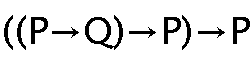
\includegraphics[scale=0.5]{pics/IMCSPeirce0}}\qquad
\fbox{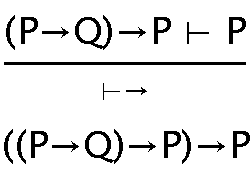
\includegraphics[scale=0.5]{pics/IMCSPeirce1}}\qquad
\fbox{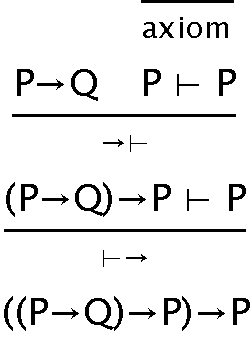
\includegraphics[scale=0.5]{pics/IMCSPeirce2}}\qquad
\caption{No Peirce's law in the intuitionistic multiple-conclusion sequent calculus}
\label{fig:IMCSPeirce}
\end{figure}


\section{The intuitionistic multiple-conclusion sequent calculus}

The rules of the intuitionistic multiple-conclusion sequent calculus aren't simply additive, but they use little more than specialised weakening. The calculus is just that of \chapref{sequentcalculus}, with different definitions of a few rules, shown in \tabref{IMCSrules}. These are defined in the file \texttt{IMCS.j}, which you can load after \texttt{MCS.jt} (and \begin{quote}\tt\small
RULE    "⊢¬"        FROM Γ,A ⊢                  INFER Γ ⊢ ¬A,∆\\
RULE    "¬⊢"        FROM Γ ⊢ A                  INFER Γ,¬A ⊢ ∆\\
RULE    "⊢→"        FROM Γ,A ⊢ B                INFER Γ ⊢ A→B,∆\\
RULE    "→⊢"        FROM Γ ⊢ A AND Γ,B ⊢ ∆   INFER Γ,A→B ⊢ ∆
\end{quote}
These definitions make it impossible to prove Pierce's law (see \figref{IMCSPeirce}), as you would expect.

\begin{table}
\centering
\caption{Multiplicative multiple-conclusion sequent calculus rules}
\label{tab:MMCSrules}
$\infer[\reason{axiom}]
       {A |- A} {}$
\qquad\vstrut{30pt}
$\infer[\reason{⊦∧}]
       {\Gamma,\Gamma' |- A@B,\Delta,\Delta' }
       {\Gamma  |- A,\Delta & \Gamma'  |- B,\Delta' }$
\qquad\vstrut{30pt}
$\infer[\reason{∨⊦}]
       {\Gamma,\Gamma' ,A|B |- \Delta,\Delta' }
       {\Gamma,A |- \Delta & \Gamma',B |- \Delta' }$
\qquad\vstrut{30pt}
$\infer[\reason{→⊦}]
       {\Gamma,\Gamma' ,A->B |- \Delta,\Delta' }
       {\Gamma  |- A,\Delta & \Gamma',B |- \Delta' }$
\qquad\vstrut{30pt}
$\infer[\reason{cut}]
       {\Gamma,\Gamma' |- \Delta,\Delta' }
       {\Gamma  |- B,\Delta & \Gamma',B |- \Delta' }$\vstrut{30pt}
\end{table}

\begin{figure}
\centering
\fbox{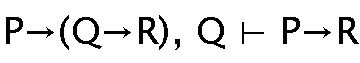
\includegraphics[scale=0.5]{pics/unifiesproviso0}}\qquad
\fbox{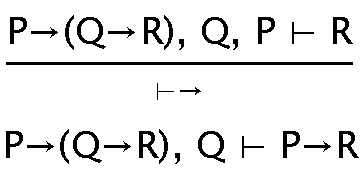
\includegraphics[scale=0.5]{pics/unifiesproviso1}}\qquad
\fbox{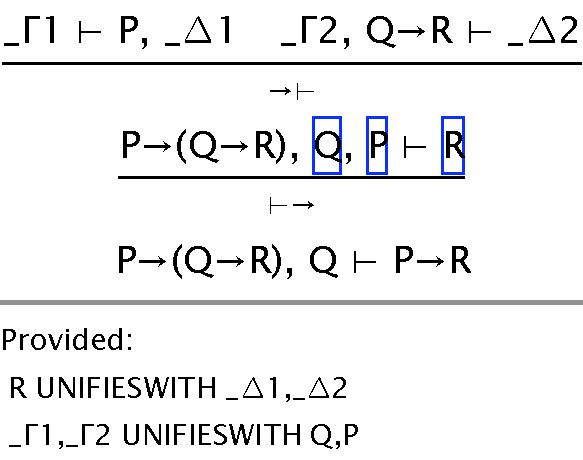
\includegraphics[scale=0.5]{pics/unifiesproviso2}}\qquad
\caption{A proof in which contexts split}
\label{fig:unifiesproviso}
\end{figure}


\begin{figure}
\centering
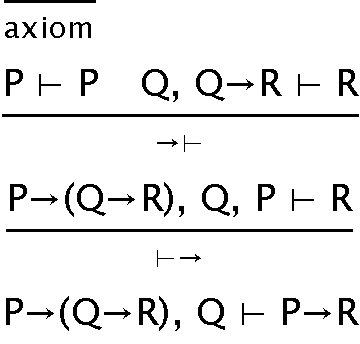
\includegraphics[scale=0.5]{pics/unifiesprovisoresolved}
\caption{Context split resolved by axiom}
\label{fig:unifiesprovisoresolved}
\end{figure}


\section{A multiple-conclusion sequent calculus with multiplicative rules}

The logic is just the normal multiple-conclusion calculus, with all of the branching rules written in multiplicative style; for maximum effect I chose an axiom rule which doesn't ignore unmatched conclusions. See \tabref{MMCSrules} for the altered rules. These rules are defined in MMCS.j, ready to be loaded after MCS.jt:
\begin{quote}\tt\small
RULE    axiom(A)                                    INFER A ⊢ A\\
RULE    "⊢∧"        FROM Γ1 ⊢ A,∆1 AND Γ2 ⊢ B,∆2        INFER Γ1,Γ2 ⊢ A∧B,∆1,∆2\\
RULE    "∨⊢"        FROM Γ1,A ⊢ ∆1 AND Γ2,B ⊢ ∆2        INFER Γ1,Γ2,A∨B ⊢ ∆1,∆2\\
RULE    "→⊢"        FROM Γ1 ⊢ A,∆1 AND Γ2,B ⊢ ∆2        INFER Γ1,Γ2,A→B ⊢ ∆1,∆2\\
RULE    "⊢≡"        FROM Γ1 ⊢ A→B,∆1 AND Γ2 ⊢ B→A,∆2  INFER Γ1,Γ2 ⊢ A≡B,∆1,∆2\\
RULE    cut(A)        FROM Γ1 ⊢ A,∆1 AND Γ2,A ⊢ ∆2        INFER Γ1,Γ2 ⊢ ∆1,∆2
\end{quote}

Since I have redefined cut, I have to redeclare its r\^{o}le to Jape:
\begin{quote}\tt\small
STRUCTURERULE CUT                   cut /* cos it's different now */
\end{quote}

When you use a multiplicative rule in this encoding, the left and right contexts split. Jape automatically records this fact in a \textsc{unifieswith} proviso, as shown in the last step of \figref{unifiesproviso}. In this simple example we have to decide whether to send $P$ and $Q$ into \_Γ1 or \_Γ2, $R$ into \_Δ1 or \_Δ2. The axiom rule of this encoding was designed to help: select $P$ in the left antecedent and apply axiom, to produce the result shown in \figref{unifiesprovisoresolved}.

\begin{figure}
\centering
\fbox{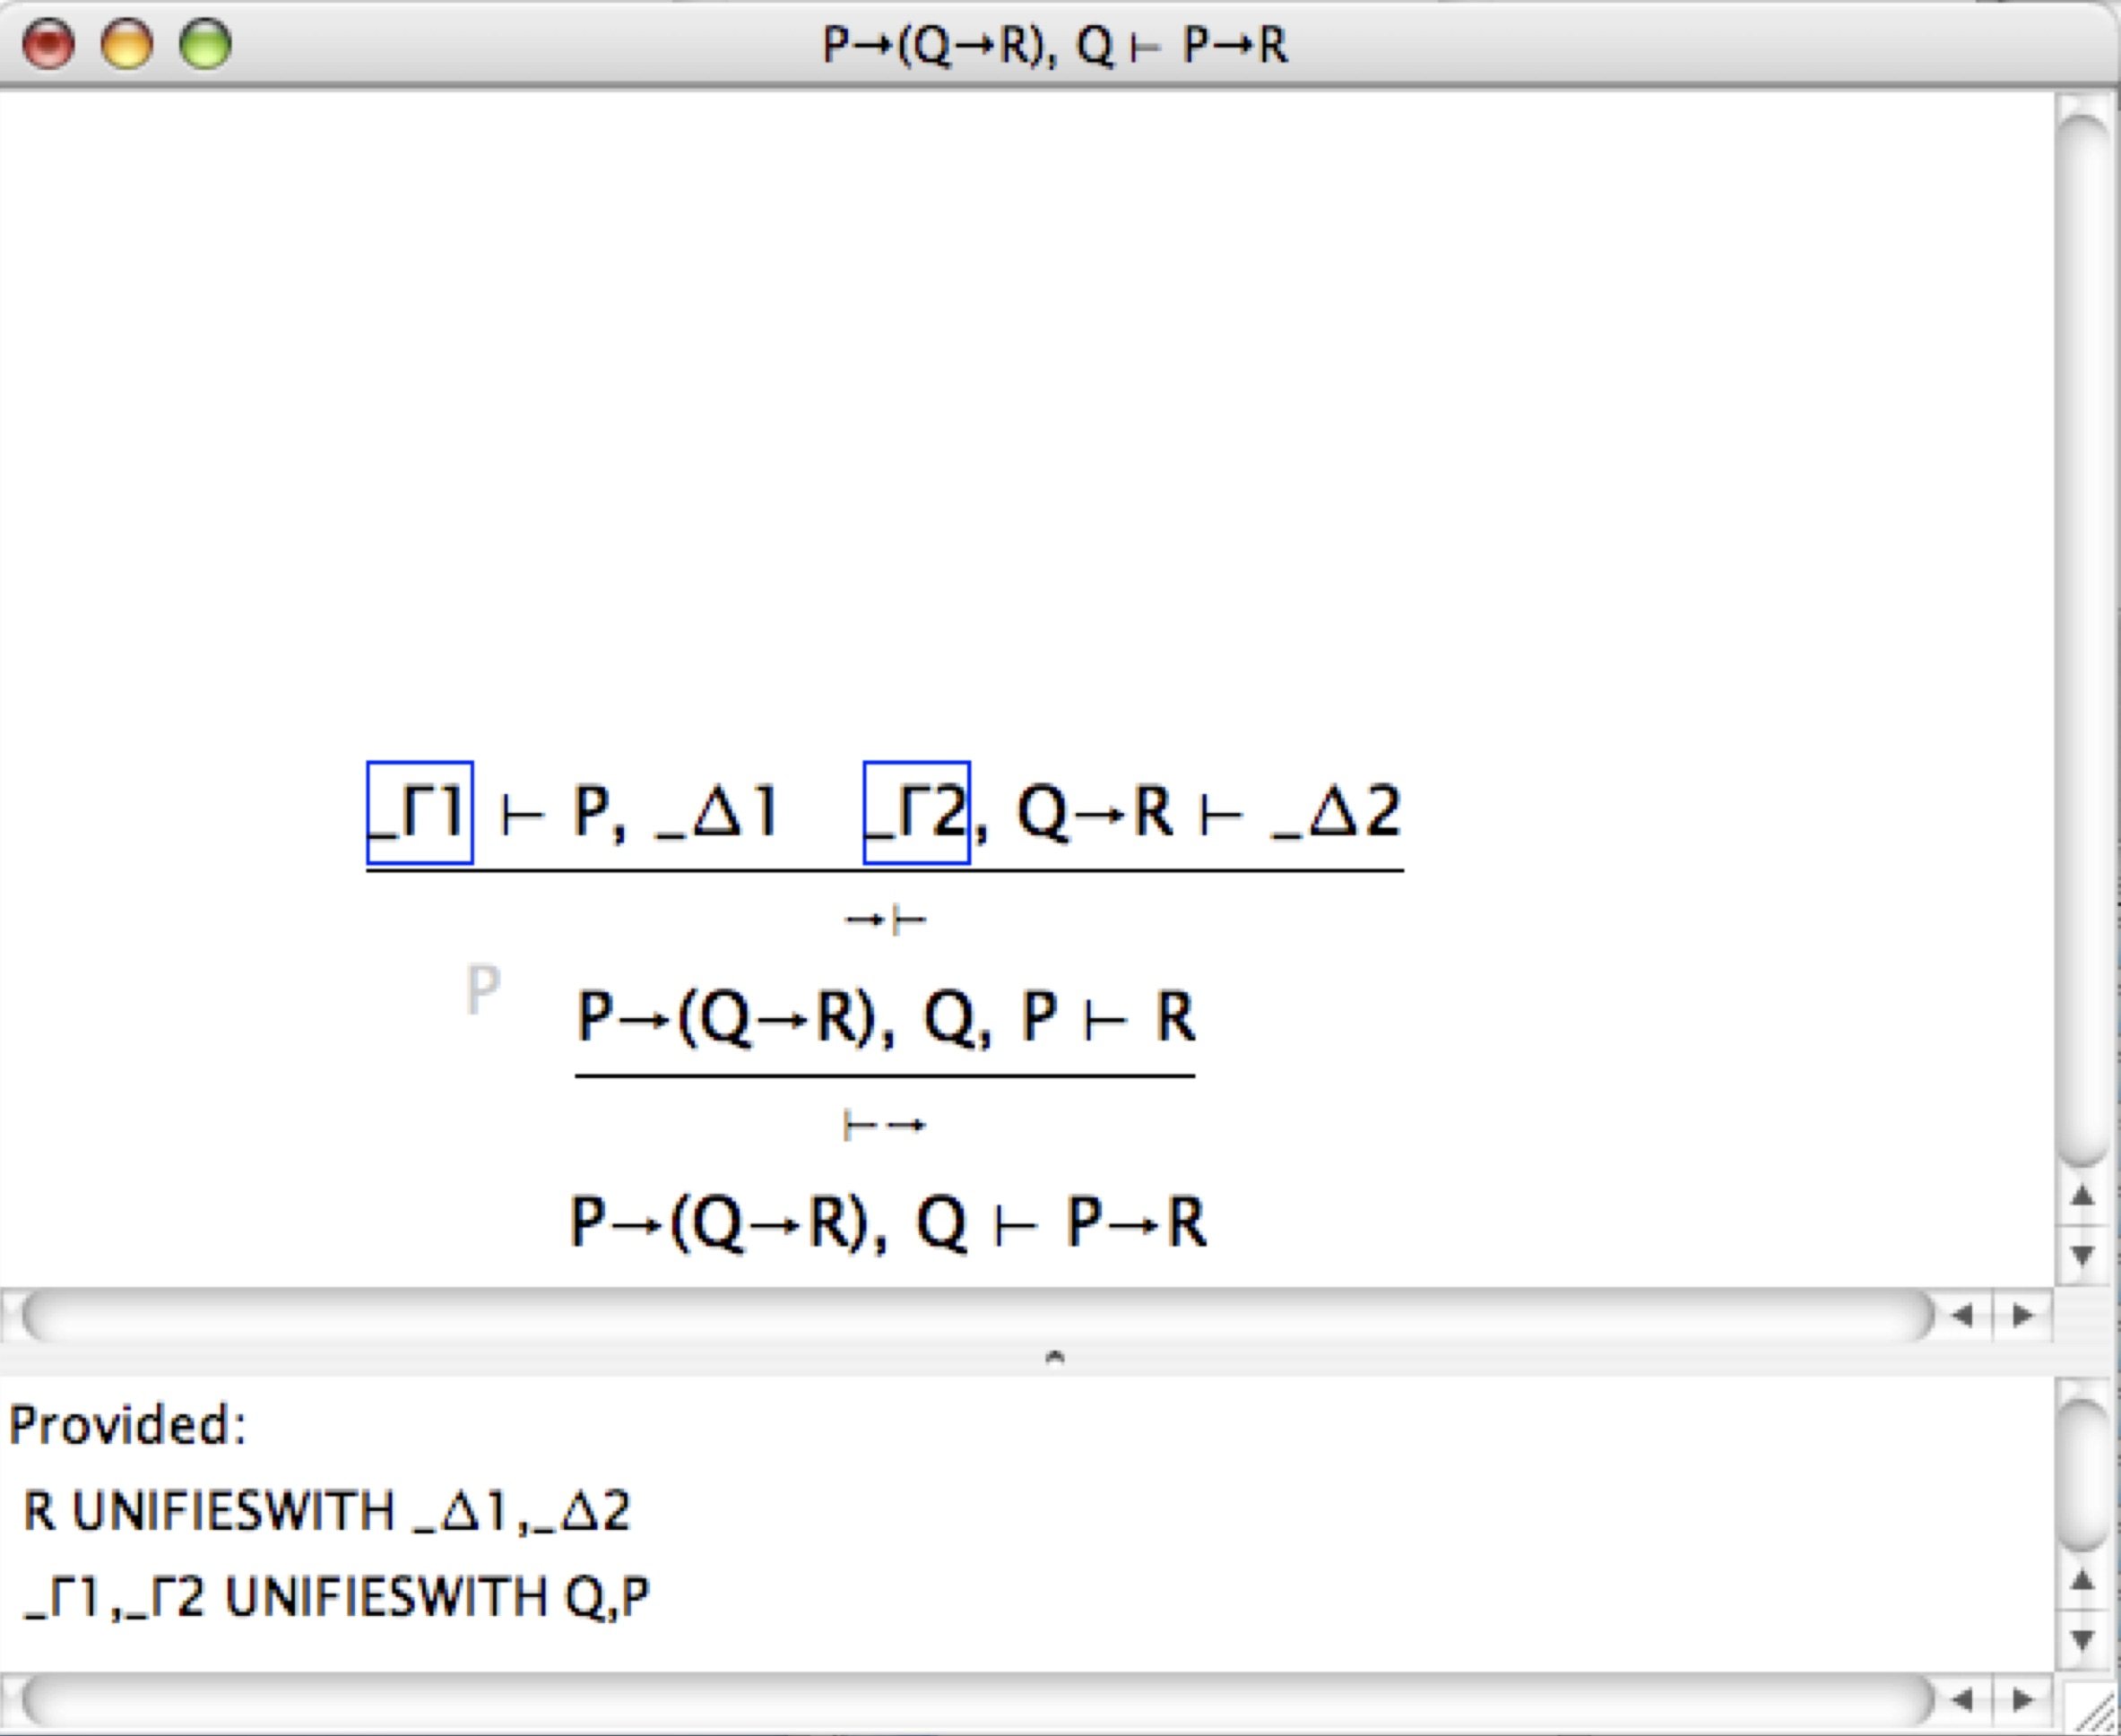
\includegraphics[scale=0.07]{pics/dragstage1.jpg}}\\
\fbox{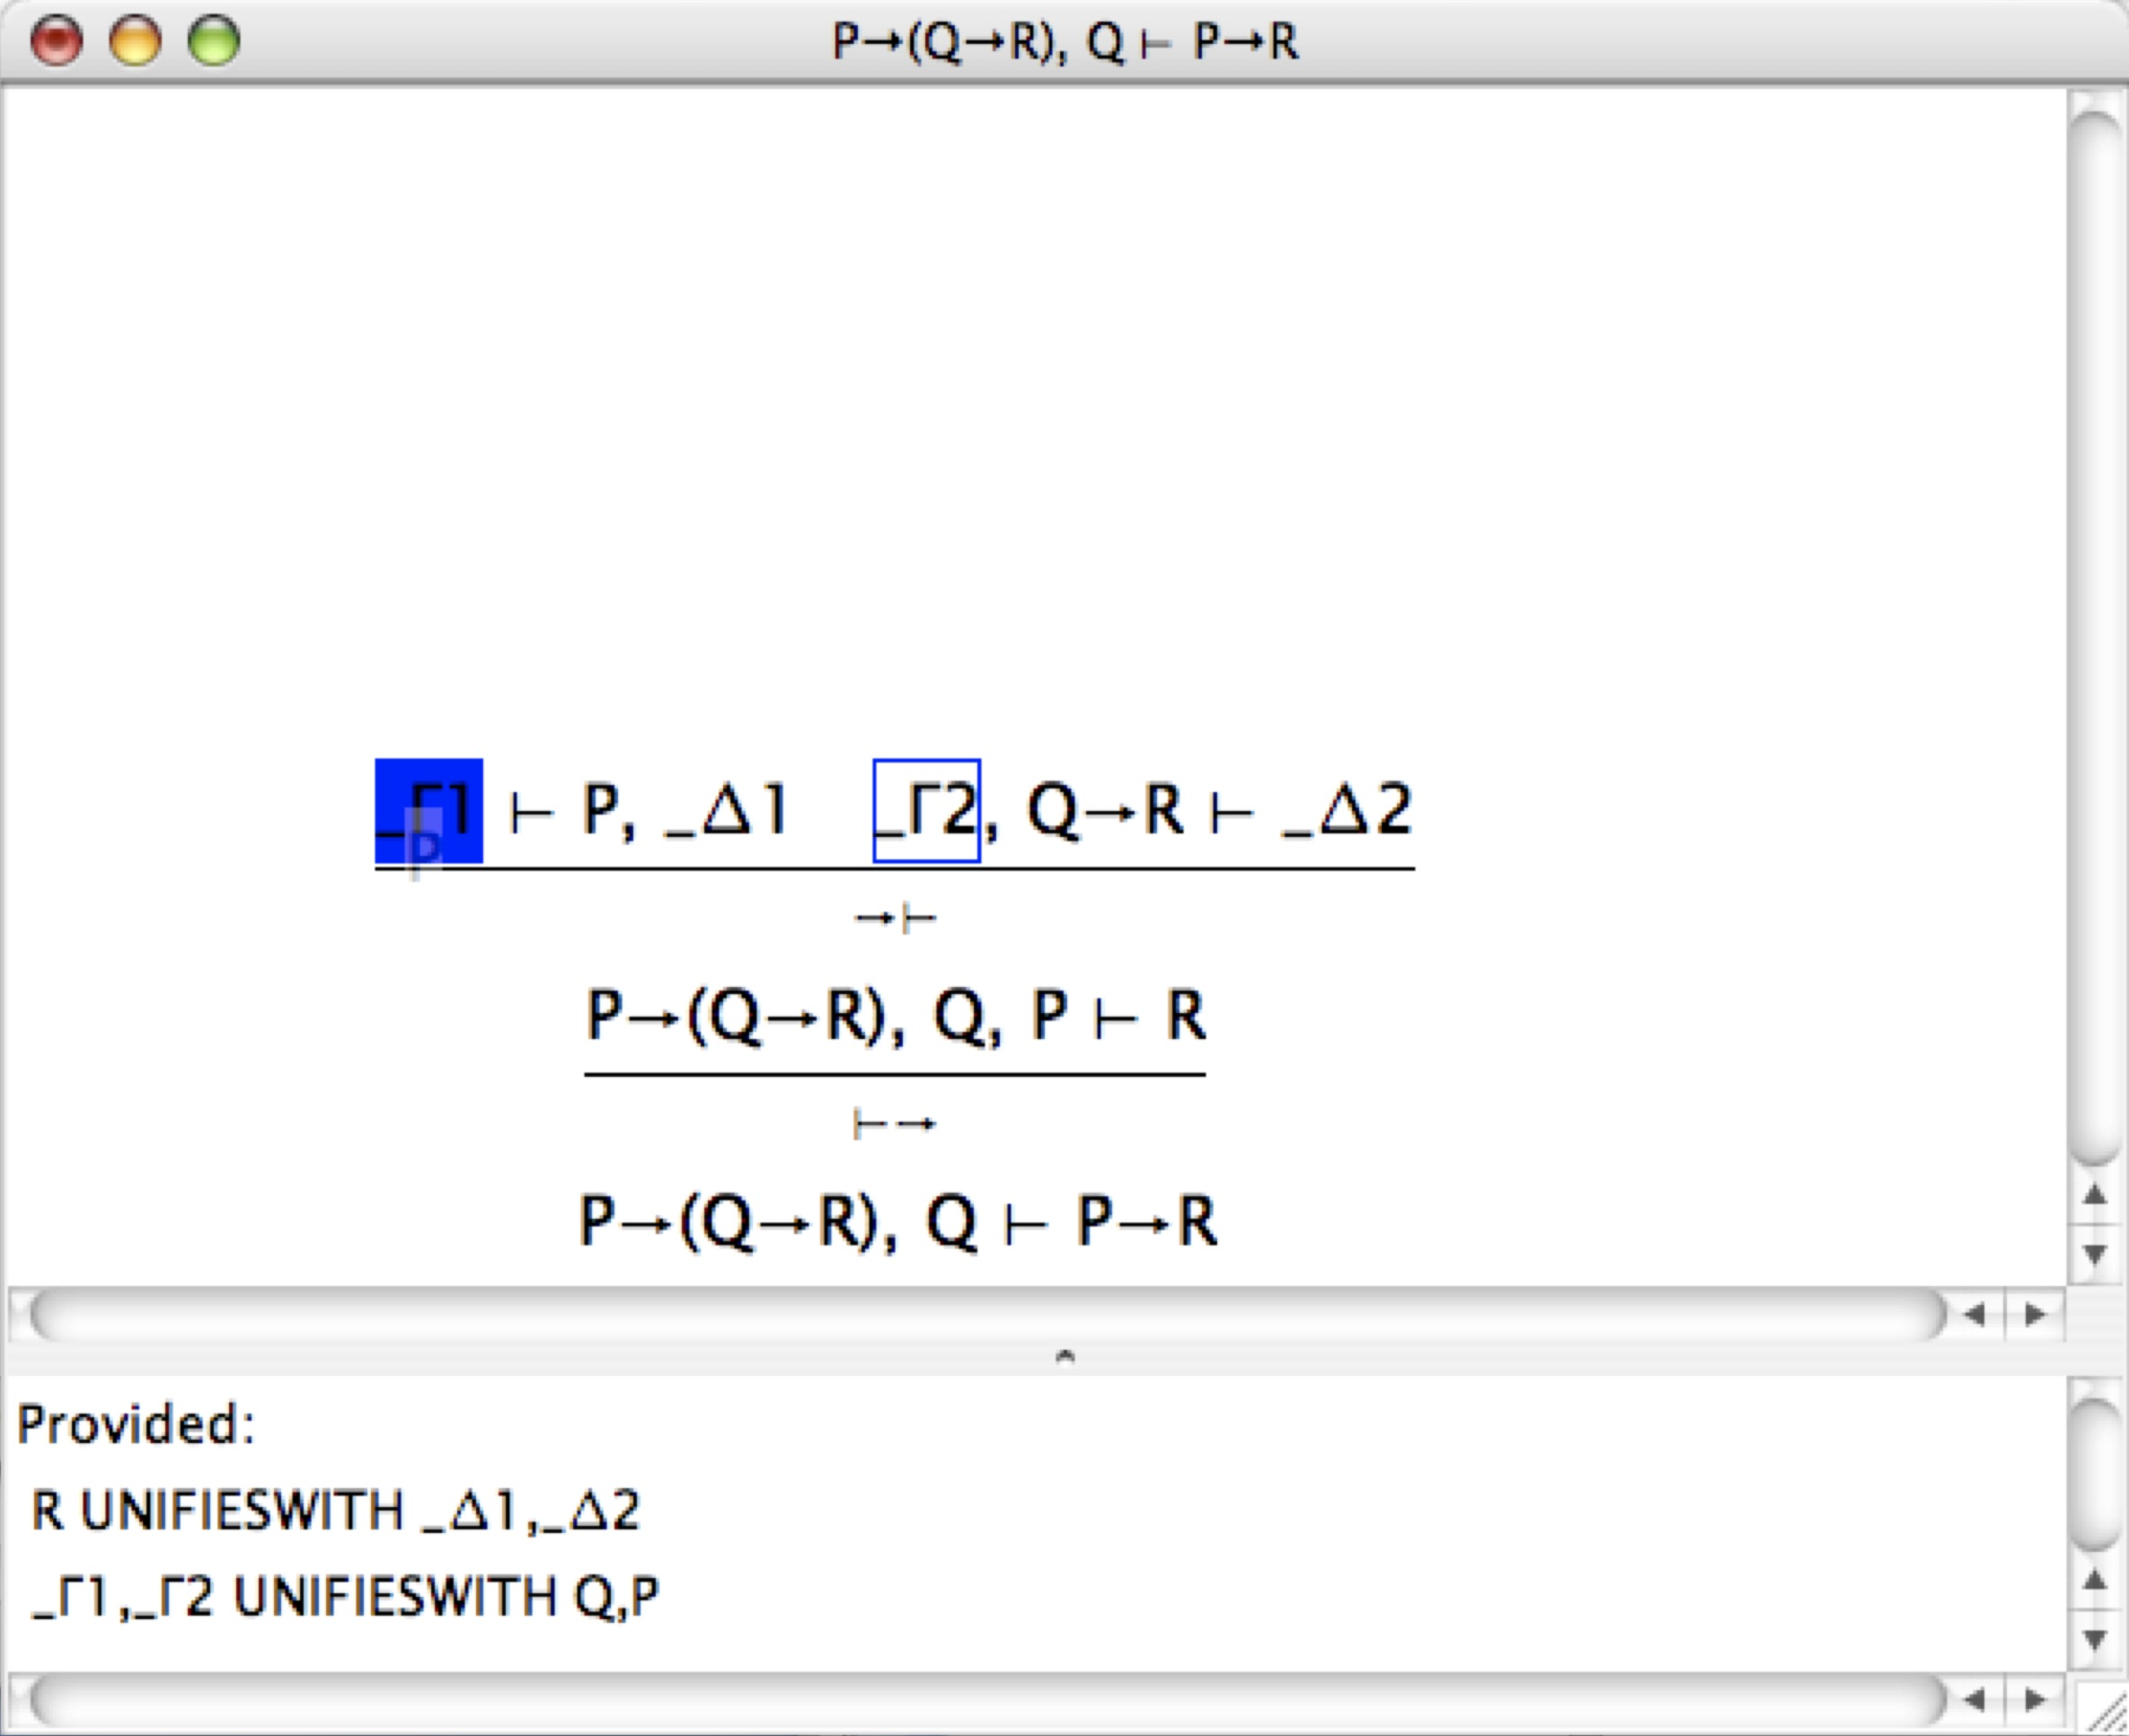
\includegraphics[scale=0.07]{pics/dragstage2.jpg}}\\
\fbox{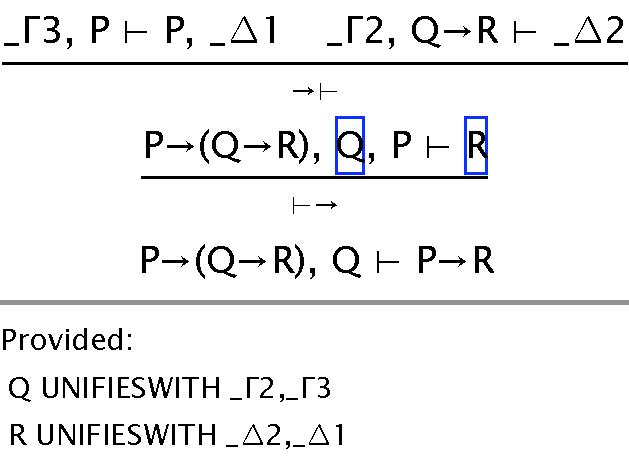
\includegraphics[scale=0.5]{pics/dragstage3}}
\caption{Resolving a context split with drag-and-drop}
\label{fig:dragstages}
\end{figure}


\textit{Resolving context-splits with drag-and-drop}

Three of the formulae in the last frame of \figref{unifiesproviso} are outlined in blue. That indicates that they are candidates for dragging into destination segment-variables. If you press and drag on the outlined instance of $P$, for example, the outlining changes to show valid drag destinations, as shown in the first frame of \figref{dragstages}. In the second frame we see how highlighting changes again when $P$ is dragged over a valid destination, and the third frame shows the effect of dropping $P$ there. Dragging $Q$ into \_Γ2 and $R$ into \_Δ2 resolves the split completely.

A similar technique can be used with rules that involve explicit weakening.


\section{Modal logic}

I intended to enhance Jape to deal with modal and linear logic. The drag-and-drop gesture, I imagined, would be part of the solution. Not so: not all the parts of a modal context split appear in the antecedents, so they wouldn't be in the proof window. And I never quite managed to wrestle the unifier into the shape it would need to deal with modal unifications. So it didn't happen as promised.


\section{Single-conclusion sequent calculus (the intuitionistic fragment)}

This was the first logic encoding that Jape ran, built by Bernard Sufrin and me in 1992. The encoding is in the file \texttt{examples/SCS.jt}.

\subsection{Inference rules}

Apart from the treatment of negation, these are a pretty ordinary selection. As with the multiple-conclusion calculus, we have chosen to use a hypothesis rule which ignores additional hypotheses, and we have made the left-hand side of a sequent a bag of formulae. The rules are very similar to those of \chapref{sequentcalculus} with Δs deleted or replaced by a formula variable $C$. In our encoding the right-hand side of a sequent contains exactly one formula --- Jape can't yet handle sequents with at most one formula on the right-hand side --- and we give rules for negation --- Jape can't yet handle definitional equality. 

Negation is often described by defining it to be equivalent to implication of absurdity: that is, $!x$ is just a way of writing $x->\bot$. Jape can't handle definitional equality, and therefore we give rules which implement that equality. The rules in \texttt{SCS\_rules.j} are
\begin{quote}\tt\small
RULE    hyp(A)                          INFER Γ,A ⊢ A\\
RULE    "⊢∧"    FROM Γ ⊢ A AND Γ ⊢ B    INFER Γ ⊢ A∧B\\
RULE    "∧⊢"    FROM Γ, A, B ⊢ C                INFER Γ, A∧B ⊢ C\\
RULE    "⊢∨(L)"     FROM  Γ ⊢ A         INFER Γ ⊢ A∨B\\
RULE    "⊢∨(R)"     FROM  Γ ⊢ B         INFER Γ ⊢ A∨B\\
RULE    "∨⊢"    FROM Γ, A ⊢ C AND Γ, B ⊢ C      INFER Γ, A∨B ⊢ C\\
RULE    "⊢¬"    FROM Γ ⊢ A→ ⊥           INFER Γ ⊢ ¬A\\
RULE    "¬⊢"    FROM Γ, A→ ⊥ ⊢ B                INFER Γ, ¬A ⊢ B\\
RULE    "⊢→"    FROM Γ, A ⊢ B           INFER Γ ⊢ A→B\\
RULE    "→⊢"    FROM Γ ⊢ A AND Γ, B ⊢ C INFER Γ, A→B ⊢ C\\
RULE    "⊢≡"    FROM Γ ⊢ A→B AND Γ ⊢ B→A        INFER Γ ⊢ A≡B\\
RULE    "≡⊢"    FROM Γ, A→B,  B→A ⊢ C   INFER Γ, A≡B ⊢ C\\
RULE    "⊥⊢"                            INFER Γ, ⊥ ⊢ A\\
RULE    "⊢∀"(OBJECT m) WHERE FRESH m\\
\tab            FROM Γ ⊢ P(m)           INFER Γ ⊢ ∀x.P(x)\\
RULE    "∀⊢"(B)     FROM Γ, P(B) ⊢ C            INFER Γ, ∀x.P(x) ⊢ C\\
RULE    "⊢∃"(B)     FROM Γ ⊢ P(B)               INFER Γ ⊢ ∃x.P(x)\\
RULE    "∃⊢"(OBJECT m) WHERE FRESH m\\
\tab              FROM  Γ, P(m) ⊢ C               INFER Γ, ∃x.P(x) ⊢ C\\
RULE    cut(A)  FROM Γ ⊢ A AND Γ, A ⊢ C INFER Γ ⊢ C\\
RULE    thin(A)     FROM Γ ⊢ B          INFER Γ, A ⊢ B\\
RULE    dup(A)  FROM Γ, A, A ⊢ B                INFER Γ, A ⊢ B
\end{quote}

\subsection{LF-style variables}

There is an encoding of an LF-style treatment of variables in the file \texttt{SCS\_LF.j}. It's identical to the treatment of variables in the multiple-conclusion calculus, with the Δ symbol deleted.

\subsection{Syntax}

Formula syntax, and use of names, is exactly as in the multiple-conclusion sequent calculus (they share the \texttt{sequent\_syntax.j} file).

Jape can't at present be configured to handle sequents with an optional formula on the right-hand side, but can deal with those with exactly one formula there. We therefore state
\begin{quote}\tt\small
SEQUENT IS BAG ⊢ FORMULA
\end{quote}

\subsection{Menus and panels}

The Rules menu is almost the same as that in the multiple-conclusion sequent calculus. The Conjectures panel is identical: the two encodings share the file \texttt{sequent\_problems.j}.

\subsection{Global variable settings}

Just as in the case of the multiple-conclusion sequent calculus, we don't want to allow the application of conjectures as if they were proved theorems and we don't want to allow the application of theorems if their hypotheses don't match.\footnote{These are pragmatic choices, driven by our expected audience of novices learning about logic. There is, of course, nothing about the logic which forces either choice.} We therefore include
\begin{quote}\tt\small
INITIALISE applyconjectures false\\
INITIALISE tryresolution false
\end{quote}

We do, however, want to allow the user to switch display modes. In place of an \textsc{initialise} directive for the \textit{displaystyle} variable, we include menu entries which control it, by inserting a radio button into the Edit menu --- one of the system menus of the Jape graphical interface. A radio button in a graphical interface is a control which has a number of mutually-exclusive settings. In a menu this appears as a number of entries, the selected one of which is ticked.
\begin{quote}\tt\small
MENU "Edit"\\
\tab RADIOBUTTON displaystyle IS\\
\tab \tab \tab "Box display"   IS box\\
\tab AND "Tree display"  IS tree\\
\tab INITIALLY tree\\
\tab END\\
END
\end{quote}
The subject of display modes is discussed in \chapref{boxNtree}.

